\documentclass[tikz]{standalone}
\begin{document}
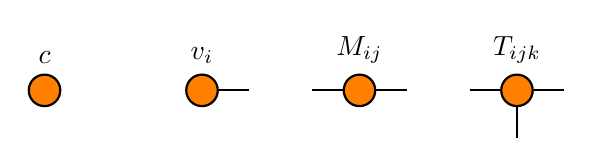
\begin{tikzpicture}
  \def\tensorsize{0.4cm}
  \tikzstyle{tensor} = [circle, draw, fill=orange, thick, inner sep = 0pt, minimum size = \tensorsize]

  \begin{scope}
    \node[tensor] (x) [label={$c$}] at (0, 0) {};
  \end{scope}

  \begin{scope}[shift={(2,0)}]
    \node[tensor] (v) [label={$v_i$}] at (0, 0) {};
    \draw[thick] (v) -- (1.5*\tensorsize, 0);
  \end{scope}

  \begin{scope}[shift={(4,0)}]
    \node[tensor] (M) [label={$M_{i j}$}] at (0, 0) {};
    \draw[thick] (M) -- (-1.5*\tensorsize, 0);
    \draw[thick] (M) -- (1.5*\tensorsize, 0);
  \end{scope}

  \begin{scope}[shift={(6, 0)}]
    \node[tensor] (T) [label={$T_{i j k}$}] at (0, 0) {};
    \draw[thick] (T) -- (-1.5*\tensorsize, 0);
    \draw[thick] (T) -- (1.5*\tensorsize, 0);
    \draw[thick] (T) -- (0, -1.5*\tensorsize);
  \end{scope}



\end{tikzpicture}
\end{document}
